\begin{frame} % Слайд 1
    \begin{center}
        \small
        Волгоградский Государственный Технический Университет \\
        Факультет электроники и вычислительной техники \\
        Кафедра САПРиПК \\
        \vspace{1.5cm}
        \normalsize
        \textbf{Метод кластеризации предпочтений жителей города по
        перемещению.}\\
        \vspace{1.0cm}
        \raggedleft\small
        \textbf{Исполнитель:}\\Чечеткин~И.~А.\\
        \textbf{Руководитель:}\\Щербаков~М.~В.\\
        \vspace{1.5cm}
        \vspace{\fill}
        \centeringВолгоград \the\year
    \end{center}
\end{frame}

\begin{frame} % Слайд 2
    \frametitle{Формулировка проблемы}
    \textbf{Актуальность.} В настоящее время формирование маршрутов в городской
    среде осуществляется на основе положений, заложенных в городской план
    развития. Обычно, эта информация достаточно устаревшая и не учитывает
    предпочтения жителей. На основе данных о предпочтениях жителей требуется
    разработать эффективный метод кластеризации предпочтений жителей города
    по перемещению.\\
    \textbf{Объект исследования} -- предпочтения жителей города, выраженные
      в географических координатах.\\
    \textbf{Предмет исследования} -- методы кластеризации предпочтений жителей.
\end{frame}

\begin{frame} % Слайд 3
    \frametitle{Цели и задачи}
    \textbf{Цель работы} -- разработка метода кластеризации предпочтений
    жителей для минимизации дискомфорта перемещения в городе.\\
    \textbf{Теоретические задачи:}
    \begin{itemize}
        \item разработка алгоритма кластеризации;
        \item разработка метода учета географических особенностей местности;
        \item разработка критериев для оценки качества кластеризации.
    \end{itemize}
    \textbf{Практические задачи:}
    \begin{itemize}
        \item генерация исходных данных;
        \item реализация разработанных алгоритмов и методов;
        \item построение полученных результатов на карте;
        \item оценка качества кластеризации.
    \end{itemize}
\end{frame}

\begin{frame} % Слайд 4
    \frametitle{Понятийный аппарат}
    \small
    \begin{itemize}
      \itemsep-5pt
        \item \textbf{Кластер} -- объединение нескольких однородных элементов,
          которое может рассматриваться как самостоятельная единица, обладающая
          определенными свойствами;
        \item \textbf{предпочтение} -- пара узлов с определенными координатами
          и идентификатором пользователя;
        \item \textbf{node (узел)} -- точка с указанными координатами и тегами;
        \item \textbf{tag (тег)} -- пары <<ключ -- значение>>;
        \item \textbf{дискомфорт} -- совокупный параметр, определяющий время
          перемещения из начального узла в конечный;
        \item \textbf{центроид} -- центр тяжести фигуры (геометрический центр);
        \item \textbf{метрика} -- функция, определяющая расстояние в
          метрическом пространстве.
    \end{itemize}
\end{frame}

\begin{frame} % Слайд 5
    \frametitle{Список литературы}
    \begin{itemize}
      \item\normalsize Data Clustering: A Review\\
        \tiny\url{https://www.cs.rutgers.edu/~mlittman/courses/
          lightai03/jain99data.pdf}
        \item\normalsize Алгоритмы кластеризации на службе Data Mining\\
          \tiny\url{http://www.basegroup.ru/library/analysis/clusterization/datamining/}
        \item\normalsize Генетические алгоритмы\\
            \tiny\url{http://mathmod.aspu.ru/images/File/ebooks/GAfinal.pdf}
        \item\normalsize Кластеризация: алгоритмы k-means и c-means\\
          \tiny\url{http://habrahabr.ru/post/67078/}
        \item\normalsize Лекции по алгоритмам кластеризации и многомерного
          шкалирования\\
          \tiny\url{http://www.ccas.ru/voron/download/Clustering.pdf}
        \item\normalsize Обзор алгоритмов кластеризации числовых пространств
          данных\\
          \tiny\url{http://habrahabr.ru/post/164417/}
        \item\normalsize Современные тенденции в кластерном анализе\\
          \tiny\url{http://www.ict.edu.ru/ft/005638/62315e1-st02.pdf}
    \end{itemize}
\end{frame}

\begin{frame} % Слайд 6
    \frametitle{Прототип}
    Псевдокод алгоритма кластеризации:\\
    \vspace{1em}
      \footnotesize
      \textbf{ВВОД} точки, границы, количество\_кластеров,\\
        \hspace{.15cm}количество\_итераций\\
      итерация = 0, пред.\_центроиды = []\\
      текущ.\_центроиды = [ГПСЧ(границы)] * количество\_кластеров\\
      \textbf{ДЕЛАТЬ ПОКА} итерация < количество\_итераций
        || \\ \hspace{.15cm} пред.\_центроиды != текущ.\_центроиды:\\
        \hspace{.5cm}\textbf{РАССЧИТАТЬ} принадлежность\_точек(точки,\\
          \hspace{.65cm} текущ.\_центроиды)\\
        \hspace{.5cm} пред.\_центроиды = текущ.\_центроиды\\
        \hspace{.5cm}\textbf{РАССЧИТАТЬ} текущ.\_центроиды(точки,
          текущ.\_центроиды)\\
        \hspace{.5cm} итерация += 1\\
      \textbf{ВЫВОД} текущ.\_центроиды
\end{frame}

\begin{frame} % Слайд 7
    \frametitle{Прототип}
    \begin{figure}
        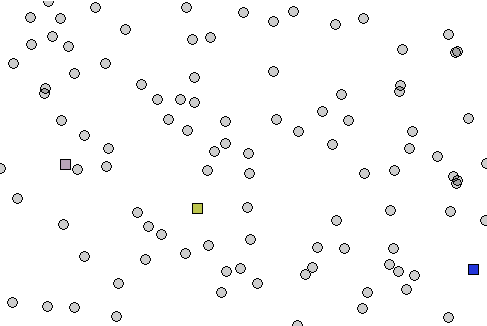
\includegraphics[width=.47\textwidth,frame]{step_0} \hfill
        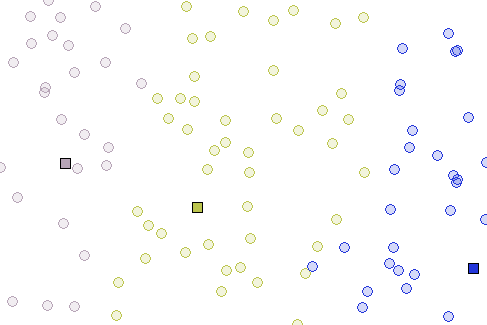
\includegraphics[width=.47\textwidth,frame]{step_1} \\
        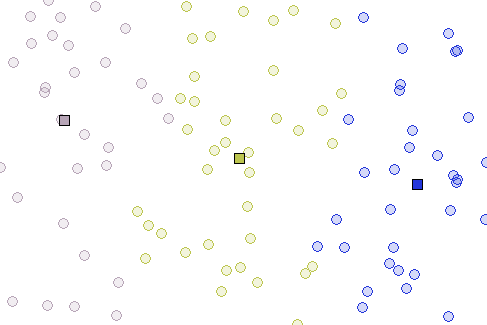
\includegraphics[width=.47\textwidth,frame]{step_2} \hfill
        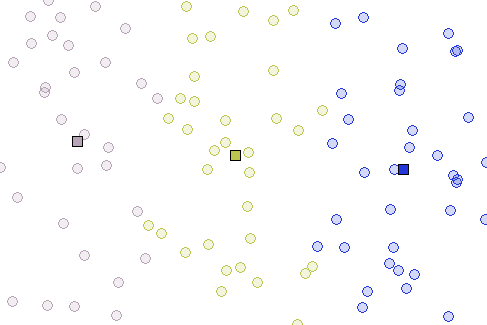
\includegraphics[width=.47\textwidth,frame]{step_6}
    \end{figure}
    \footnotesize\emph{Реализованный алгоритм:}
      \url{https://github.com/DSKarramba/clustering}\\
\end{frame}

\begin{frame} % Слайд 8
    \frametitle{Результат}
    \begin{figure}
        \center
        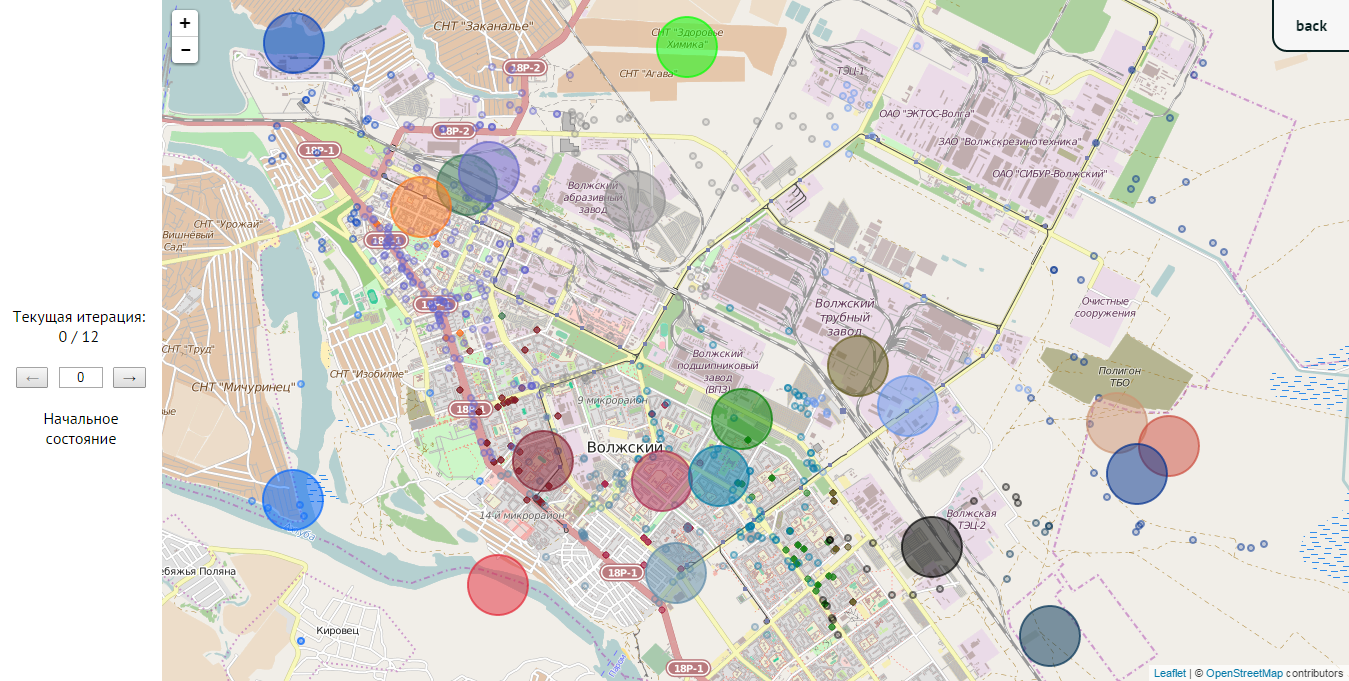
\includegraphics[width=\textwidth]{clustering_0}
    \end{figure}
    
    \vspace{5ex}
\end{frame}

\begin{frame} % Слайд 9
    \frametitle{Результат}
    \begin{figure}
        \center
        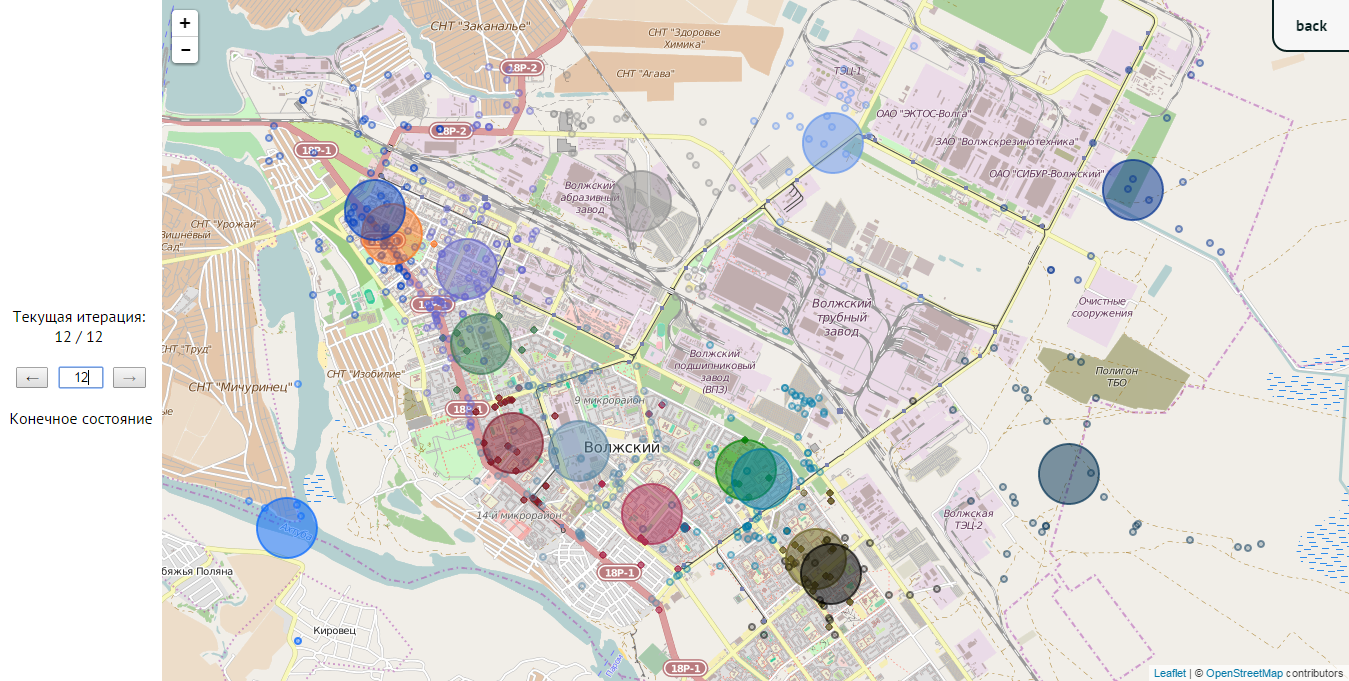
\includegraphics[width=\textwidth]{clustering_1}
    \end{figure}
    
    \footnotesize\emph{Ссылка на результат работы алгоритма:}
      \url{http://dskarramba.github.io/cluster/}
\end{frame}